\chapter{根与翼} % Introduction chapter suppressed from the table of contents

中国社会一直非常强调家庭价值观,希望实现家族的持续传承(如:四世同堂),代代相传的关系对每个家庭成员的成长产生深远影响。我们每个人都只是人类进化过程中的短暂过渡。父母普遍希望把最好的东西传承给下一代。然而,我们需要问自己,什么东西能够持久,仅仅是财富和金钱吗?

继承大量财富,但如果不懂得如何正确利用,有时可能反而会削弱个人的竞争力,并可能导致不负责任的行为,最终成为社会的蛀虫。

"七个习惯"的作者史蒂芬·柯维(Stephen
Covey)在书的结尾(最后一章)中提到,我们可以传承给下一代并具有持久价值的,只有两样东西:根和翼。

'There are only two lasting bequests we can give our children - one is
roots, the other wings.'

\hypertarget{ux6839}{%
\subsection{根}\label{ux6839}}

回看人类过去一百三十年,除了打了两次世界大战外,也做了很多前所未有的创新:

\begin{itemize}
\tightlist
\item
  电灯 (煤气灯)
\item
  汽车 (马车)
\item
  飞机
\item
  摩天大厦
\item
  半导体,集成电路
\item
  计算机
\item
  互联网
\item
  移动电话
\end{itemize}

人类创新并不仅限于前述领域,这只是我们看到的凤毛麟角,其他在医疗、电影、音乐、数学等各个领域都表现出了卓越的创新力,这些都是祖先留给我们的宝贵财富。

举例来说,如果十九世纪欧洲城市的居民能够坐上像"Back to the
Future"那样的时间跑车,见到两百年后现代人的生活,他们将感到难以置信。

然而,当我们观察现代社会的儿童和年轻人时,由于不再需要担心衣食住行,他们往往将更多的精力投入到虚拟世界的游戏、养宠物、以及在线购物等方面,这确实引发了一些担忧。

有人可能会提出反对意见,说:``我不是贝多芬,也不是乔布斯,我没有像他们那样非凡的魄力。''

\hypertarget{ux4e1cux5317ux864e}{%
\subsubsection{东北虎}\label{ux4e1cux5317ux864e}}

中国东北虎作为濒危物种,目前在国内的数量估计不超过30只,因此国家动物保护组织采取了多项措施予以保护,其中包括人工饲养。专家曾试图将这些人工饲养的东北虎重新放归野外,但这一任务极为艰巨。它们是否能够在野外独立存活下来,仍然是一个未知数。有一部纪录片生动地讲述了动物保护组织在这一过程中所面临的各种挑战和困难。\\

\framebox{%
\begin{minipage}[t]{0.97\columnwidth}\raggedright
我们经过严格的筛选,挑选出最具潜力的老虎。第一次选中的是一只年轻且体型较大的老虎,将其放到一个模拟自然环境的大型操场,供专家进行观察。刚开始,这只老虎还是表现出了典型野生老虎的特征,如:警惕地观察周围的环境等。然而,几小时后,这只老虎没有抵抗住低温环境,还是选择回到自己的巢穴,这次尝试失败了。另一只被选中的老虎虽然充满活力,也不怕冷,但却缺乏野生动物的警惕性,它已经习惯了人类的存在,这可能会给它的野外生活带来危险。因此,专家不得不放弃了这只老虎。

要确保老虎在野外的独立生存,它们必须能够自行觅食。在自然环境中,它们主要的捕猎对象就是鹿,但鹿非常敏捷,时速可达五十公里,而且具备很强的耐力。因此,专家需要评估老虎是否能够成功捕猎到鹿,否则就不能将它们放归到野外。在评估过程中,专家发现老虎的奔跑和狩猎能力明显不如野生老虎,因为缺少运动,它们缺乏狩猎的能力。因此,专家设计了多种锻炼方法,如使用车辆牵引轮胎,并插上鲜肉块来刺激它们奔跑。经过一系列的锻炼,老虎的体力得到了恢复,但能否成功捕猎到鹿仍然是未知数。

另一个试验是用汽车拖着鹿的尸体,以此吸引老虎奔跑。然而,有些老虎因为在平时的饲养过程中并没有吃过鹿肉,所以对此并不感兴趣。最终,只有两三只老虎追着汽车跑,试图抓到鹿。最后,有两只年轻的老虎获胜了。但要将鹿的尸体作为奖励喂给获胜的老虎也并不容易,发现它们对着鹿的尸体不知道如何下口,因为以前都是由饲养员将肉切好后喂给它们吃。最终,这两只老虎花了数小时才慢慢学会如何吃到鹿肉。

\strut
\end{minipage}}

看完这部纪录片,我立刻想到了有些年轻的程序员,他们也是在相对受到保护的环境下工作。这些程序员可能已习惯了管理层或经验丰富的同事对他们的代码质量要求并不高。因此,如果我们希望这些年轻的程序员注重代码质量,就跟保护区把饲养的东北虎放归野外一样,需要经过艰苦的培训,以提高他们的竞争力。管理层必须认识到,只是一味地保护程序员,对他们提供高质量的代码没有要求,那么公司的产品质量将永远无法提高,也难以与其他公司竞争。

我曾与一位企业质量官进行交流,发现越来越多的企业开始注重质量,尤其是在客户对质量要求非常高的行业,如银行、基金和保险等。他说:``公司制定质量流程非常容易,但是很多公司在执行过程中出了问题。根据我近二十年的从业经验,企业文化起着关键作用,因为提供高质量产品的核心是每个人都要具备质量意识,并将其养成习惯。

\hypertarget{ux7ffc}{%
\subsection{翼}\label{ux7ffc}}

除了根的传承,祖先还留给了我们``翅膀'',赋予了我们自由的能力,以此打破负基因的传承,追求改善、变革和创新,而不是简单地将这些基因传给下一代。

To be a powerful transition person, one must first change his inner
first.

我们每个人都只是在人类几万年进化历程中的一个瞬间。必须先从内而外做改变,才可以持久。要成为一位有影响力的过渡者,我们必须首先进行由内而外的改变,这样的改变才能持久。

当然,我们也可以在自己可控的范围内进行创新,或至少有所改善。

\hypertarget{ux98deux884cux5b9eux9a8c}{%
\subsubsection{飞行实验}\label{ux98deux884cux5b9eux9a8c}}

韦德兄弟同样需要克服许多困难。他们并非工程或数学天才,但为了实现``飞翔''的梦想,他们进行了无数次实验。最终,他们在1900年成为了世界上第一对成功的空中飞行者。

\framebox{%
\begin{minipage}[t]{0.97\columnwidth}\raggedright
韦德兄弟 (Wright brothers) 第一次飞行成功
在韦德兄弟之前,德国的飞行之父Lilienthal已经进行了大量的计算和研究,试图实现人类在空中飞行,但却没有成功。然而,这两位俄亥俄州的兄弟究竟是如何成为世界上第一个成功飞向天空的人的呢?他们回顾说:``我们需要更多的技巧而不仅仅是机器。即使没有发动机,飞行仍然是可能的,但没有必要的知识和技能肯定是无法实现的。我们试图向鸟类学习成功飞行的技巧,而不是试图挑战大自然,完全参照鸟类,像它们一样。''

韦德兄弟根据Lilienthal先生的计算结果,在风洞里进行实验,发现他的计算存在错误。他们发现鸟类在飞行时会使用翅膀的尖端来控制方向。此外,他们发现,为了平衡飞机在机体旋转而产生的扭矩,会使飞机向反方向转动,影响飞行。飞行是在不稳定的大气条件下操控不稳定的机器,充满了许多变数,因此非常困难。最终,韦德兄弟抛弃了所有错误知识,通过不断的实验,自己发明了飞机的重要部件,包括翅膀、舵、发动机、螺旋桨等,还研究了它们之间是如何相互影响的。

开始的时候,飞行只延续了十二秒钟。两年后,它可以在空中半个小时以上。

%\href{文件:1903wrightScreenshot_2022-02-14_103500.jpg}{300px}\\
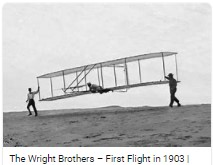
\includegraphics[width=6cm]{1903wrightScreenshot_2022-02-14_103500.jpg}\\
\strut
\end{minipage}}

\hypertarget{ux603bux7ed3}{%
\subsection{总结}\label{ux603bux7ed3}}

针对软件开发,我们这一代继承了之前从60年代以来的各种硬件软件的创新,
给予我们继续发展的根。

敏捷宣言指出了传统瀑布式开发和传统计划驱动开发的弊端,给我们以``翼'',为有能力的团队提供了机会,可以更快速地开发出高质量的产品。

提升质量和效率是一个逐步改进的过程。例如,我们已经从过去的主观定性判断过渡到以数据说话,通过分析缺陷数据以支持决策,开始采用定量管理的方法。通过多轮迭代数据的收集和分析,逐渐建立标杆,更好地提升质量和效率。

团队和企业要健康成长依赖以下主要因素(与上一章创新的要素类似):

\begin{itemize}
\tightlist
\item
  团队成员的能力与动力

  \begin{itemize}
  \tightlist
  \item
    个人提升、自我管理、代码质量等部分能帮助提升
  \end{itemize}
\item
  改进要有专注

  \begin{itemize}
  \tightlist
  \item
    例如针对如何减少缺陷返工,尽早在评审和前期测试发现缺陷,如何做好迭代回顾部分能帮助团队了解应如何开始
  \end{itemize}
\item
  高层要制定高的目标,也要提供资源

  \begin{itemize}
  \tightlist
  \item
    可参考开始过程改进之旅里面的获取高层支持,尽早估算改进能节省多少成本,要求立项,把过程改进作为项目来管理
  \end{itemize}
\end{itemize}

团队的持续改进至关重要。这样,即使在未来遇到像前言中提到的那位严格的技术总监------陈总,也能避免被挑出一大堆毛病了。

相反,如果一家软件开发公司只注重项目的按时交付、追求急功近利,而忽视了产品质量,结果将导致不断出现问题和返工,最终会被那些持续改进的竞争对手抛在后头。

预祝你们公司会成为软件开发的丰田!

\begin{description}
\item[]
\begin{description}
\tightlist
\item[]
-\/-\/-===\textless{}\textless{}\textless{} END
\textgreater{}\textgreater{}\textgreater{}===-\/-\/-
\end{description}
\end{description}


